
\section{Technique}
\label{sec:approach}



We next describe our SQL query synthesis technique in details.
How to infer the desirable query for the examples
shown in Section~\ref{sec:example} will
be discussed thoroughly in this section.

\begin{figure}[t]
  \centering
  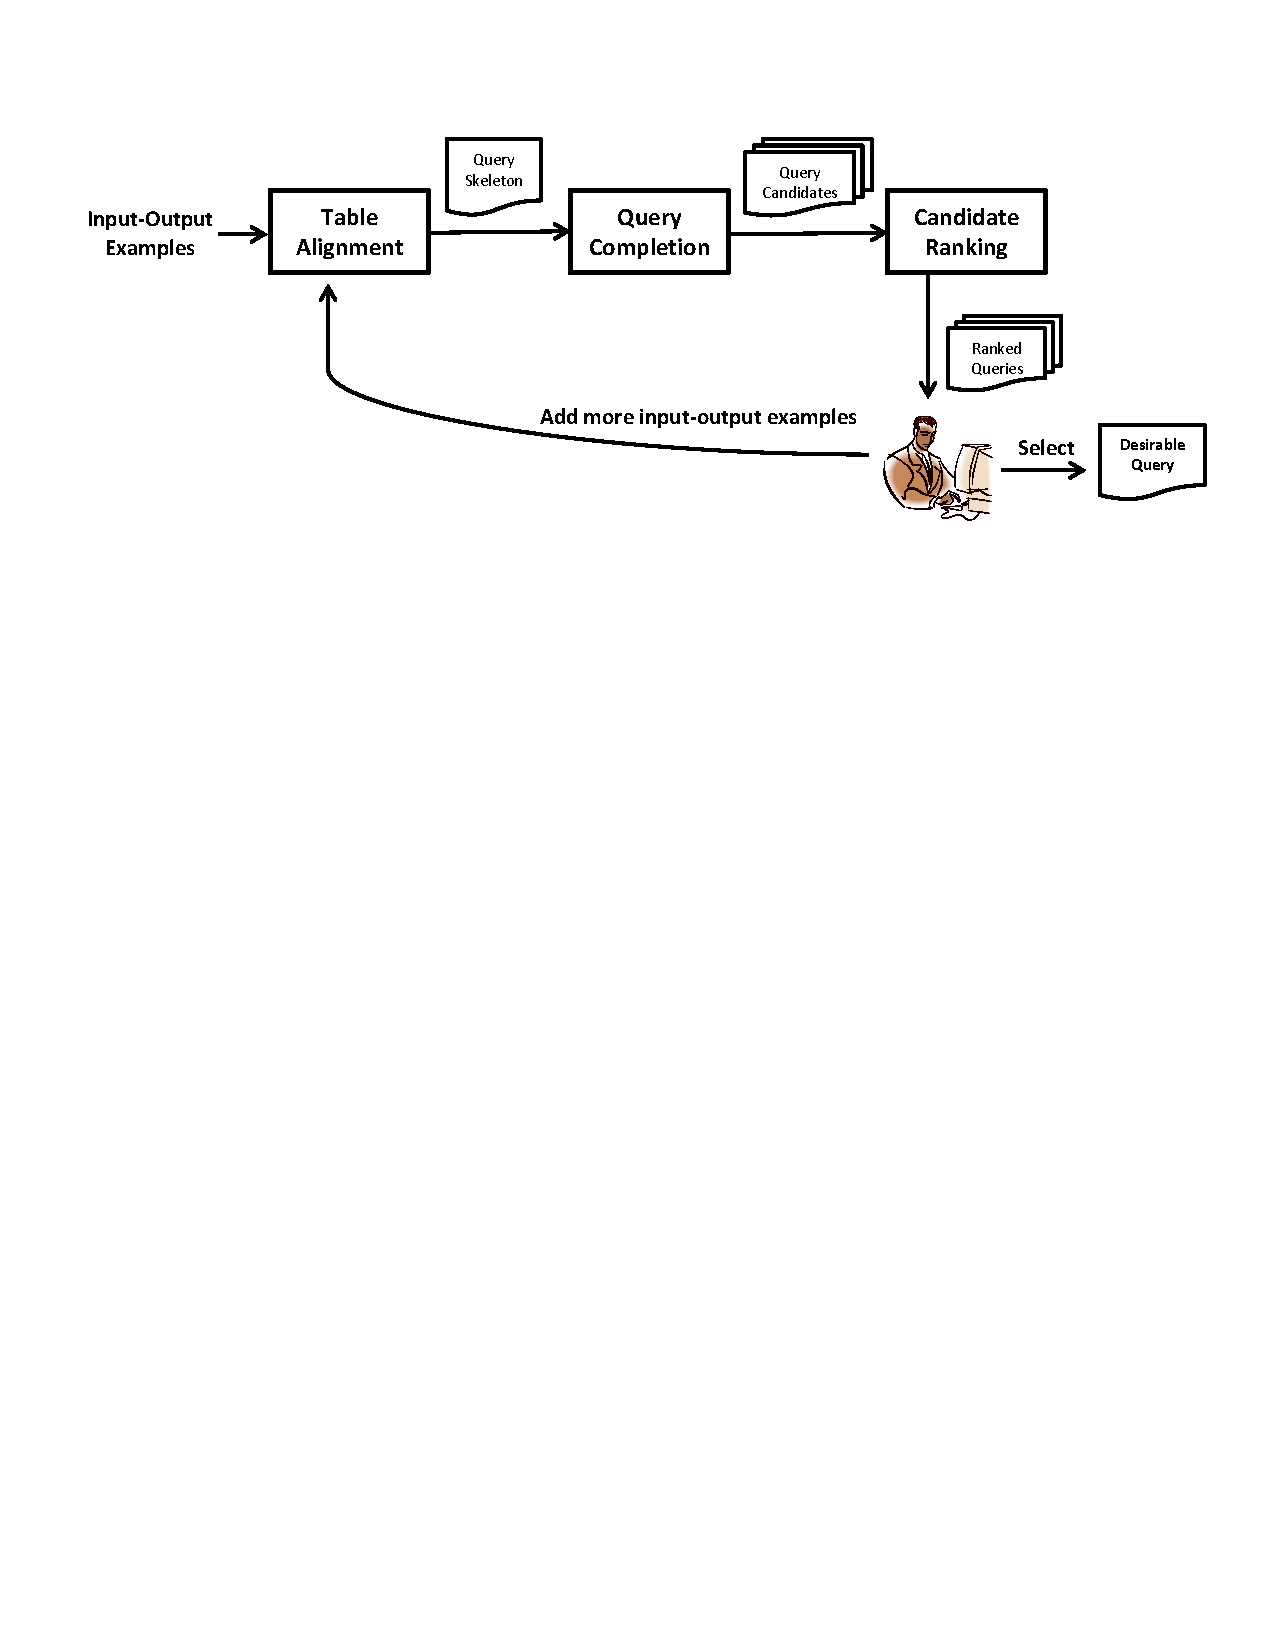
\includegraphics[scale=0.53]{workflow}
  \vspace*{-5.0ex}\caption {{\label{fig:workflow} The workflow of our SQL query synthesis approach.
}}

\end{figure}

\subsection{Overview}
Figure~\ref{fig:workflow} sketches the general workflow of our technique.

At a high level, our technique consists of three major steps: Query Skeleton
Creation(Section~\ref{sec:skeleton}), SQL Query Completion
(Section~\ref{sec:completion}), and Query Candidate Ranking (Section~\ref{sec:ranking}).
Specifically, our approach takes from users input-output examples. It first infers
a partially-complete query skeleton. The inferred query skeleton, though contains
incomplete parts as holes, serves as good guidance for synthesizing a complete SQL query.
Our approach next uses two techniques to fulfill a SQL skeleton. It first
uses decision-tree learning to learn possible query conditions (Section~\ref{}), and
 employs type-directed search to figure out possible aggregates (Section~\ref{}).
After the SQL Query Completion step, our approach produces a list of syntactically-valid
query candidates that satisfy the provided input-output examples.
However, it is possible that multiple query candidates can be synthesized based on the
provided input-output example. To deal with that, our approach ranks all generated candidates,
and provides users a ranked list of SQL queries with the most useful ones on the top. 
%This makes our tool more usable.


End-users can use our approach to obtain SQL query to transform
multiple, huge database tables by constructing small, representative
input and output example tables. On some examples, we speculate
that our approach
may produce a SQL query that satisfies the input and output examples
given by the user, but does not address the intention
that the user wants. To address this issue, we adapt a simple
interaction model from~\cite{Harris:2011} to ask users to investigate the results of
an output SQL query and report any discrepancy. In this case,
the user can refine the inferred SQL query by providing a more
informative input-output example (or multiple input-output examples
that together describe the required behavior) that demonstrate the behavior on
which the originally-inferred SQL query behaves incorrectly.

\subsection{Query Skeleton Creation}
\label{sec:skeleton}

In this step, our technique scans the provided input and output examples, guesses
what a target SQL query might look like, and infers a set of query skeletons
that capture the basic query structures.

A query skeleton is an incomplete SQL query, which
captures three basic query structures that could
often be decided after a simple scan over the examples:
tables used in a result SQL
query, table columns used to join input tables, and table
columns for projecting the query results. Other parts in a SQL query such as conditions
(including selection and having conditions), and aggregates
are left as unkown, and will be determinated in the next step (Section~\ref{sec:completion}).



%\begin{itemize}

%\item
\vspace{1mm}
\noindent \textit{\textbf{Step 1: Determining the Table Set.}} 
In practice, end-users are unwilling to provide more than enough
inputs. Therefore, every input table specified in the example
is expected to be used to construct a desirable SQL query.
Based on this observation, we assume that every input table
should be used as least once in the query. By default, the
table set $T$ used in the result SQL query contains all given input tables.
However, it is possible that a single table will be used for multiple times.
Our technique does not forbid this case, rather, we adopt a single heuristic
to estimate the used table set: if the same column from an input table appears more than once in the
example output, we add the input table the same number of times to the used table set.

%we view it as a strong indicator that this table will be joined multiple times and add it to our table
%set $T$ using an alias.


%\item
\vspace{1mm}
\noindent\textit{\textbf{Step 2: Determining Joining Columns. }} Given two arbitrary tables, there exist many
ways to join them. Enumerating all possible joining conditions may introduce a huge number of joining
conditions and would quickly become intractable. We observe that, in practice, two tables are often joined via the following
three cases: (1) tables are joined on their primary keys with the same (or compatible) data types, such
as joining a \textit{student} table with an \textit{enrollment} table with the \textit{student\_id} column. It does not
make any sense to join two tables on a Integer column and a String column. (2) tables are joined
using columns with the same name, such as joining a \textit{student} table with a \textit{enrollment} table on the
\textit{student\_name} column. and (3) two columns that have the data type, and have a large portion of
overlapped values in their corresponding input tables can be used as a joining condition. It is straightforward to check the first 
two cases to identify possible joining columns. For the third case, our technique scans the given input tables to check ``value similarity''
between two arbitrary columns, and selects columns whose ``value similarity'' is above a fixed threshold as joining columns.

%\item
\vspace{1mm}
\noindent \textit{\textbf{Step 3: Determining Output Columns.}} To identify output table columns on
which the querying result would be projected, our technique checks whether each output
table column name appears in any input tables. If so, we used the matched column
from the input table as the output column. Otherwise, the output column
must be produced by using aggregation. Our technique keeps track of those aggregation columns
and search for proper aggregates in the next phase (Section~\ref{sec:agg_search}). 

%After determining the table set and joining columns,
%the next step is to identify potential column names on which the result would be projected. If a
%column in the output table  does not appear in any input table's column list, this output column must
%be produced by aggregation. Our algorithm keeps track of these columns and appends a \CodeIn{group by} ... \CodeIn{having} ...
%clause to the query skeleton.

%\end{itemize}
\vspace{1mm}

In summary, this step infers three parts as a query skeleton: tables used in constructing a SQL query, joining conditions
to connect the input tables, and a list of columns to project the output results.

%It is worth noting that the results obtained from the above steps are not \textit{safe} in
%terms that they may miss some valid SQL queries. 

%We made the above assumption for the sake of tractability,
%since in theory, the bound of table number in a SQL query is $O(n_t!)$, where $n_t$ is the number of given tables;
%while the bound of possible number of join is $O(c_t^2)$ and the bound of the number of conditions is $O(n_t!n_tc_t^2)<O(n_t^3c_t^2)$.

%\subsubsection{Inferring Output Table Schema}

%Lacks schema

\subsubsection{Example}

For our motivating example, from the output table (Figure~\ref{tbl:output}), our technique identifies that
column {\CodeIn{Student\_name}} comes from table \CodeIn{student} and
column {\CodeIn{Max\_Score}} is a new one which must be created by using aggregation.
% which indicates aggregation and group by.

%while the bound of possible number of join is $O(c_t^2)$ and the bound of the number of conditions is $O(n_t!n_tc_t^2)<O(n_t^3c_t^2)$.

\begin{figure}[t]
	\centering
%\begin{CodeOut}
%\begin{alltt}
%\textbf{select student.Student\_name, $\color{blue}{<Aggregate>}$ 
%from student, enrolled
%where student.Student\_key = course.Student\_key
%      and \color{red}{<Conditions>}
%group by student.Student\_key
%having \color{red}{<Conditions>}}
%\end{alltt}
%\end{CodeOut}
%\vspace{-5mm}
		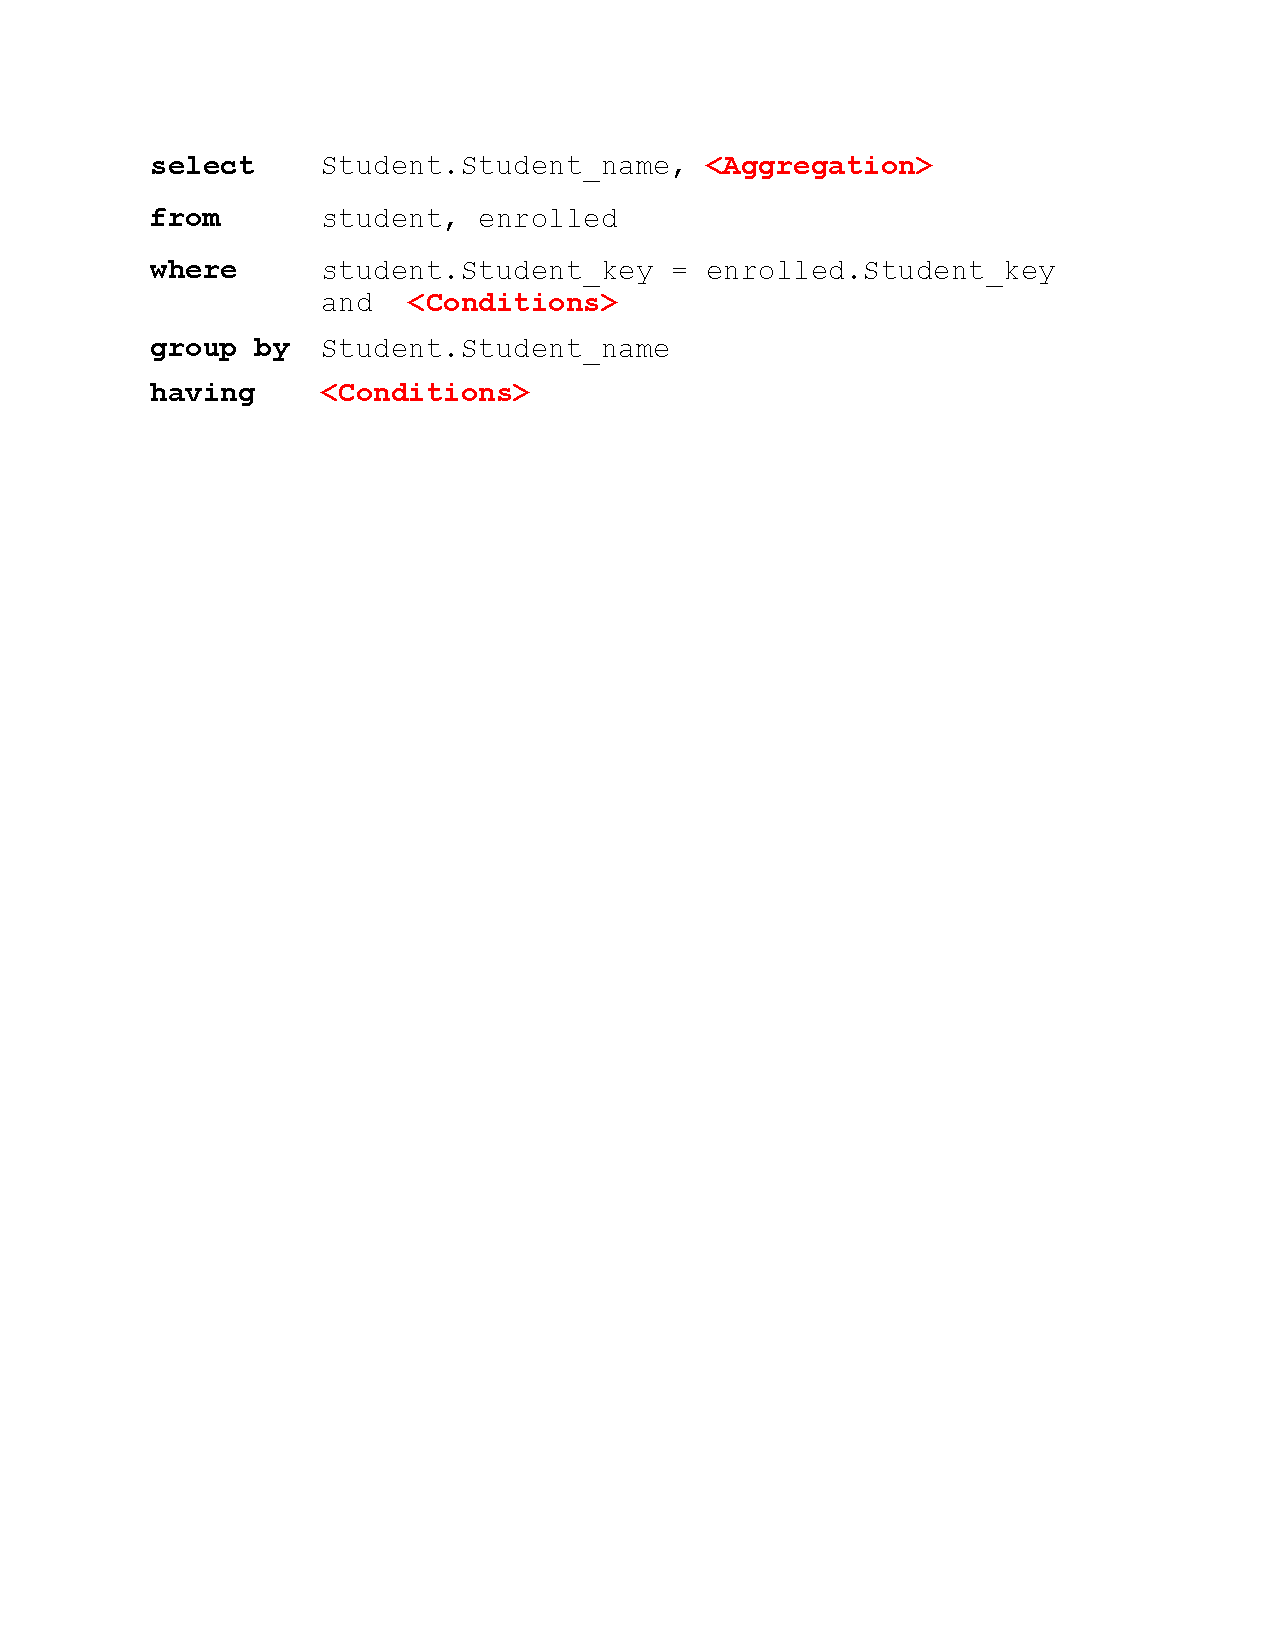
\includegraphics[width=0.4\textwidth]{sql_skeleton.pdf}
	\caption{The SQL skeleton created for the motivating example
in Section~\ref{sec:example}.}
	\label{fig:skeleton}
\end{figure}

The created query skeleton  is shown in Figure \ref{fig:skeleton}.
As we can see from Figure \ref{fig:skeleton},  there are three unknown structures represented
by $<$Aggregation$>$ or $<$Conditions$>$ in red color, which will be filled in the next phase.


\subsection{Query Completion}
\label{sec:completion}

\begin{figure*}[t]
    \centering
    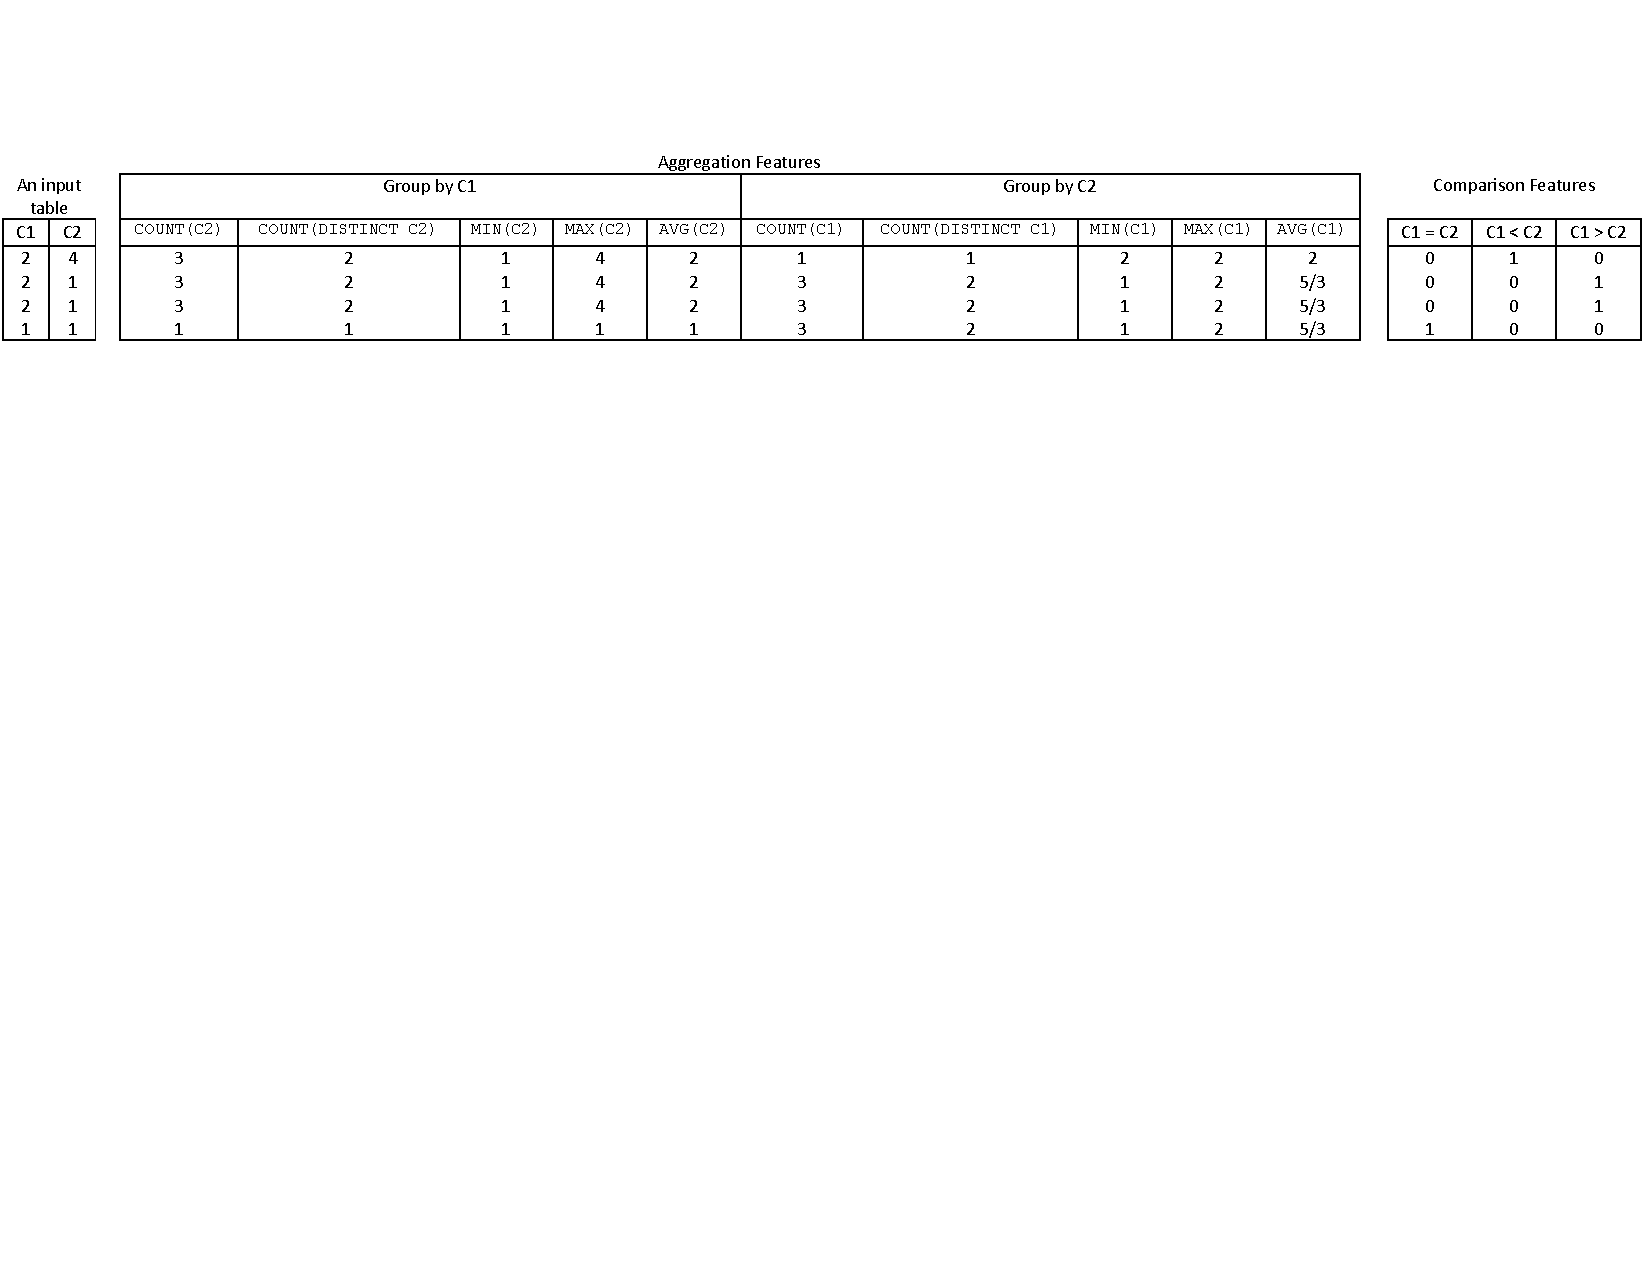
\includegraphics[scale=0.68]{featurex}
    \vspace{-7mm}
	\caption{Illustration of two additional features
    added by \ourtool. (Left) An example input table with
    two columns: C1 and C2. (Center) The aggregation features added by
    \ourtool for the input table. (Right) The comparison features
    added by \ourtool for the input table.
    Take the first row in the input table as an example,
    when grouping the table by column C1 (with value 2), the number
    of values in the C2 column is 3; the  number of
    distinct values in the C2 column is 2; the minimal value
    in the C2 column is 1, the maximal value in the C2 column
    is 4, and the average value in the C2 column is 2. Similar
    results can be computed if the table is grouped by the C2
    column.
}
	\label{fig:features}
\end{figure*}


In this step, \ourtool analyzes each created query skeleton
, and completes the missing query conditions, the
\CodeIn{GROUP BY} and \CodeIn{HAVING} clause (Section~\ref{sec:condition}),
aggregates (Section~\ref{sec:agg_search}), and
the \CodeIn{ORDER BY} clause (Section~\ref{sec:orderby}).
\ourtool outputs a list of syntactically-correct SQL queries
that satisfy the given example input and output.


%The SQL skeleton produced by the first step, though incomplete,
%serves as a good reference in inferring complete and valid SQL queries.
%In this step, our technique the remaining incomplete parts: conditions and
%aggregates, by rule-based learning and type-directed search, respectively.

\subsubsection{Inferring Query Conditions}
\label{sec:condition}

\ourtool casts the problem of \textit{inferring query conditions} as
 \textit{learning appropriate rules} that can perfectly divide a search space
into a positive part and a negative part. In our context, the search space
is all tuples from joining all query tables; the positive part
includes all tuples in the output table; and the negative part includes the rest
tuples.

The standard way for rule learning is using a decision-tree-based
algorithm. However, how to design a good features
becomes a key challenge.
Existing approaches~\cite{Tran:2009} simply use
tuple values in the input table(s) as features, 
and limits their abilities in inferring more
complex rules as query conditions. In particular,
merely using tuple values as features can only infer
conditions that compares a column value with a constant
(e.g., \CodeIn{student.level = 'senior'}), but
fails to infer conditions using aggregates (e.g., \CodeIn{COUNT(enrolled.course\_id) > 2}),
or conditions comparing the values of two table columns
(e.g., \CodeIn{enrolled.course\_id > enrolled.score}).



\ourtool addresses this challenge by adding two types of
additional features to each tuple, and uses
the existing tuple values together with the additional features
for rule learning.

\begin{itemize}

\item {\textbf{Aggregation Features}}. For each
column in an input table, \ourtool tries
to group all table data by \textit{each} tuple's
value, then applies every applicable aggregate (i.e.,
\CodeIn{COUNT}, \CodeIn{COUNT DISTINCT}, \CodeIn{MAX},
\CodeIn{MIN}, and \CodeIn{AVG} for a numeric type column;
and \CodeIn{COUNT}, and \CodeIn{COUNT DISTINCT} for
a string type column) to every
 \textit{remaining} column for computing the aggregation result. 
The ``Aggregation Features'' part in Figure~\ref{fig:features}
shows an example.

\item {\textbf{Comparison Features}}. For each tuple,
\ourtool compares
the values of every two type-comparable columns, and records
the comparison results ($1$ or $0$) as features.
The ``Comparison Features'' part in Figure~\ref{fig:features}
shows an example.

\end{itemize}

%The above two additional features seamlessly encodes SQL
%structure
% knowledge encoding permits our technique
%to make use of correlations between columns, rather than only values
%from each isolated and sequential columns.
%Table~\ref{tbl:com} shows an example.


%Using both tuple values and the enhanced features,
\ourtool employs a variant of the decision tree algorithm,
called PART~\cite{Frank:1998}, to learn a set of rules
as query conditions.
PART has two notable advantages over the
original decision tree algorithm~\cite{Quinlan:1986}.
First, it uses a ``divide-and-conquer'' strategy to repeatedly
build rules and remove data instances (i.e., tuples) that have already been covered until
no more data instances are left, and thus is faster.
Second, PART less memory, since it builds a decision
tree incrementally, prunes falsified branches on-the-fly,
and only keeps the minimal tree structure in memory.



\todo{The incerasing number of features, can be falsified quickly,
more features permits undiscover more rules}


Figure~\ref{fig:fullexample} shows an example, in
which the expected query condition uses the \CodeIn{COUNT} aggregate.


\begin{figure*}[t]
  \centering
  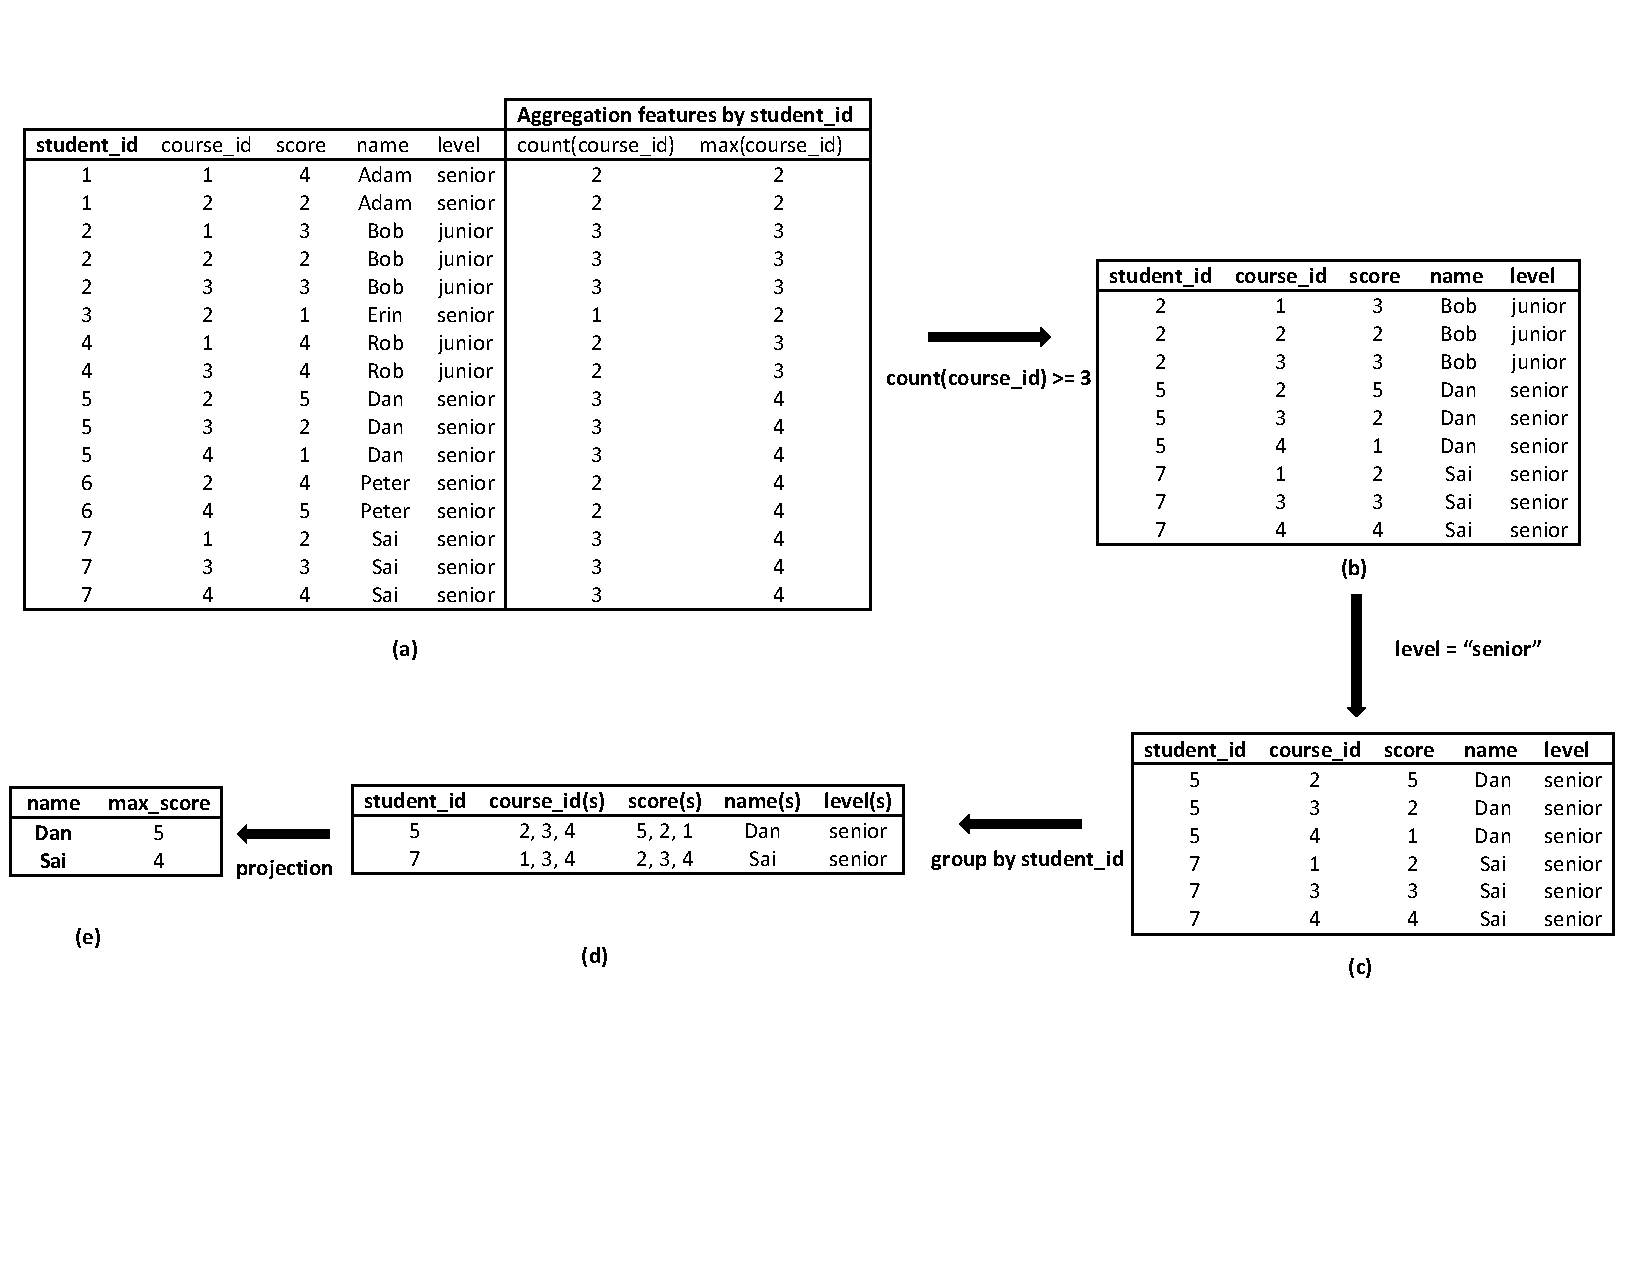
\includegraphics[scale=0.65]{fullexample}
  \vspace*{-5.0ex}\caption {{\label{fig:fullexample}
  Illustration of how additional features added by \ourtool
  helps in inferring query conditions. (a) shows \ourtool
  enriches the original table (Left: the
  result of joining table \CodeIn{student} with table
  \CodeIn{enrolled} on the \CodeIn{student\_id} column)
  with additional features. For brevity, only relevant
  aggregation features are shown. Using the added aggregation
  features, \ourtool infers two query conditions that
  transform the original table into the table show in (b).
  Note that, without the aggregation features enhanced by
  \ourtool, a learning algorithm will \textit{fail} to learn the above conditions.
  (c) shows the output table, which is produced by projecting the
   table in (b)
  on its column: name, and an aggregate: \CodeIn{MAX}(score).
}}

\end{figure*}


\ourtool next splits the learnt rules into two disjoint parts:
and put each part into its appropriate place.
Specifically, \ourtool puts conditions
using aggregates to the \CodeIn{HAVING}
clause; and puts other conditions to the \CodeIn{WHERE} clause.
This is based on the SQL language's specification:
query conditions using aggregates are valid only when they
are used \textit{after} the \CodeIn{GROUP BY} clause.
Take the conditions inferred in Figure~\ref{fig:fullexample}
as an example, \ourtool puts the query
condition: \CodeIn{student.level =`senior'}
in the \CodeIn{WHERE} clause,
puts condition: \CodeIn{COUNT(enrolled.course\_id) > 2}
in the \CodeIn{HAVING} clause, and puts
column \CodeIn{student\_id} to the \CodeIn{GROUP BY} clause.

%\smallskip





%\end{itemize}

\subsubsection{Searching for Aggregates}
\label{sec:agg_search}

For every column in the output table that has no matched
column in the input tables,
\ourtool repeatedly applies each aggregate on
every input table column; and then outputs the aggregate (with the
input table column) that produces the same output 
in the output table. To speed up the exhaustive search,
\ourtool uses two rules to filter away many infeasible
combinations.


\begin{itemize}
\item \ourtool only applies an \textit{applicable} aggregate
to a \textit{type-compatible} table column. Specifically,
the data values in an output column must be compatible with an
aggregator's return type. For instance, if an output column
contains float values, it cannot be produced by using the \CodeIn{COUNT}
or \CodeIn{COUNT DISTINCT} aggregators, or 
using the \CodeIn{MAX} aggregator over a column with integer type.
On the other hand, some aggregates cannot be applied on
table columns with certain types. For example, the \CodeIn{AVG}
aggregate cannot be applied to columns with string type.
%\ourtool encodes such knowledge to avoid unnecessary search.

\item \ourtool checks whether each value in the output
column has appeared in the input table. If not, the
output column cannot be produced by using
using the \CodeIn{MAX} and \CodeIn{MIN} aggregator.
%such as \CodeIn{MAX} and \CodeIn{min},
%is used, each value in the output column must has appeared in the input table.
\end{itemize}

%In our experience, the type-directed searching strategy significantly reduces the
%searching space and makes our tool find the desirable aggregates faster.

%\todo{Order by structure, relatively each to add}
\subsubsection{Searching for columns in the \CodeIn{ORDER BY} column}
\label{sec:orderby}
\ourtool scans the values of each column in the output table. If
the data values in a column are sorted, \ourtool
append the column name to the \CodeIn{ORDER BY} clause.


\subsection{Candidate Ranking}
\label{sec:ranking}


It is possible that multiple SQL queries satisfying
the given input-output examples will be returned.
To help end-users select their expected queries,
\ourtool ranks more likely queries higher in the output.
%This may adversely impact end-users who want to
%perform simple query tasks but now need
%to select the query of their intent.
%To alleviate this problem, 
To do so, \ourtool employs
the Occam's razor principle, which states that the
simplest explanation is usually the correct one.
A simpler query is less likely to overfit the given examples
than a complex one, even when both of them
can transform the example input to the example output.


%We define a comparison scheme between different
%SQL queries by defining a partial order between them. Some of
%these choices are subjective, but have been observed to work well.
A SQL query is simpler than another one if it uses
fewer query conditions (including conditions in the \CodeIn{HAVING}
and \CodeIn{FROM} clauses) or the expressions (including
aggregates) in each query condition or clause are pairwise simpler.
For example, expression \CodeIn{COUNT(student\_id)} is simpler than
\CodeIn{COUNT(DISTINCT student\_id)}.
Simpler query conditions and expressions often suggest the extraction logics
are more common and general.

In our implementation, \ourtool computes a cost for each
query, and prefers queries with lower costs. The cost
for a SQL query is computed by summarizing
the costs of all conditions, aggregates,
and other expressions
appearing in the \CodeIn{GROUP BY} and \CodeIn{ORDER BY} clauses.
(The cost of each condition, aggregate and expression
is approximated by its length.)
%This heuristic has been observed
%to work well.
Figure~\ref{fig:rank} shows an example.


\begin{figure}[t]
\centering
 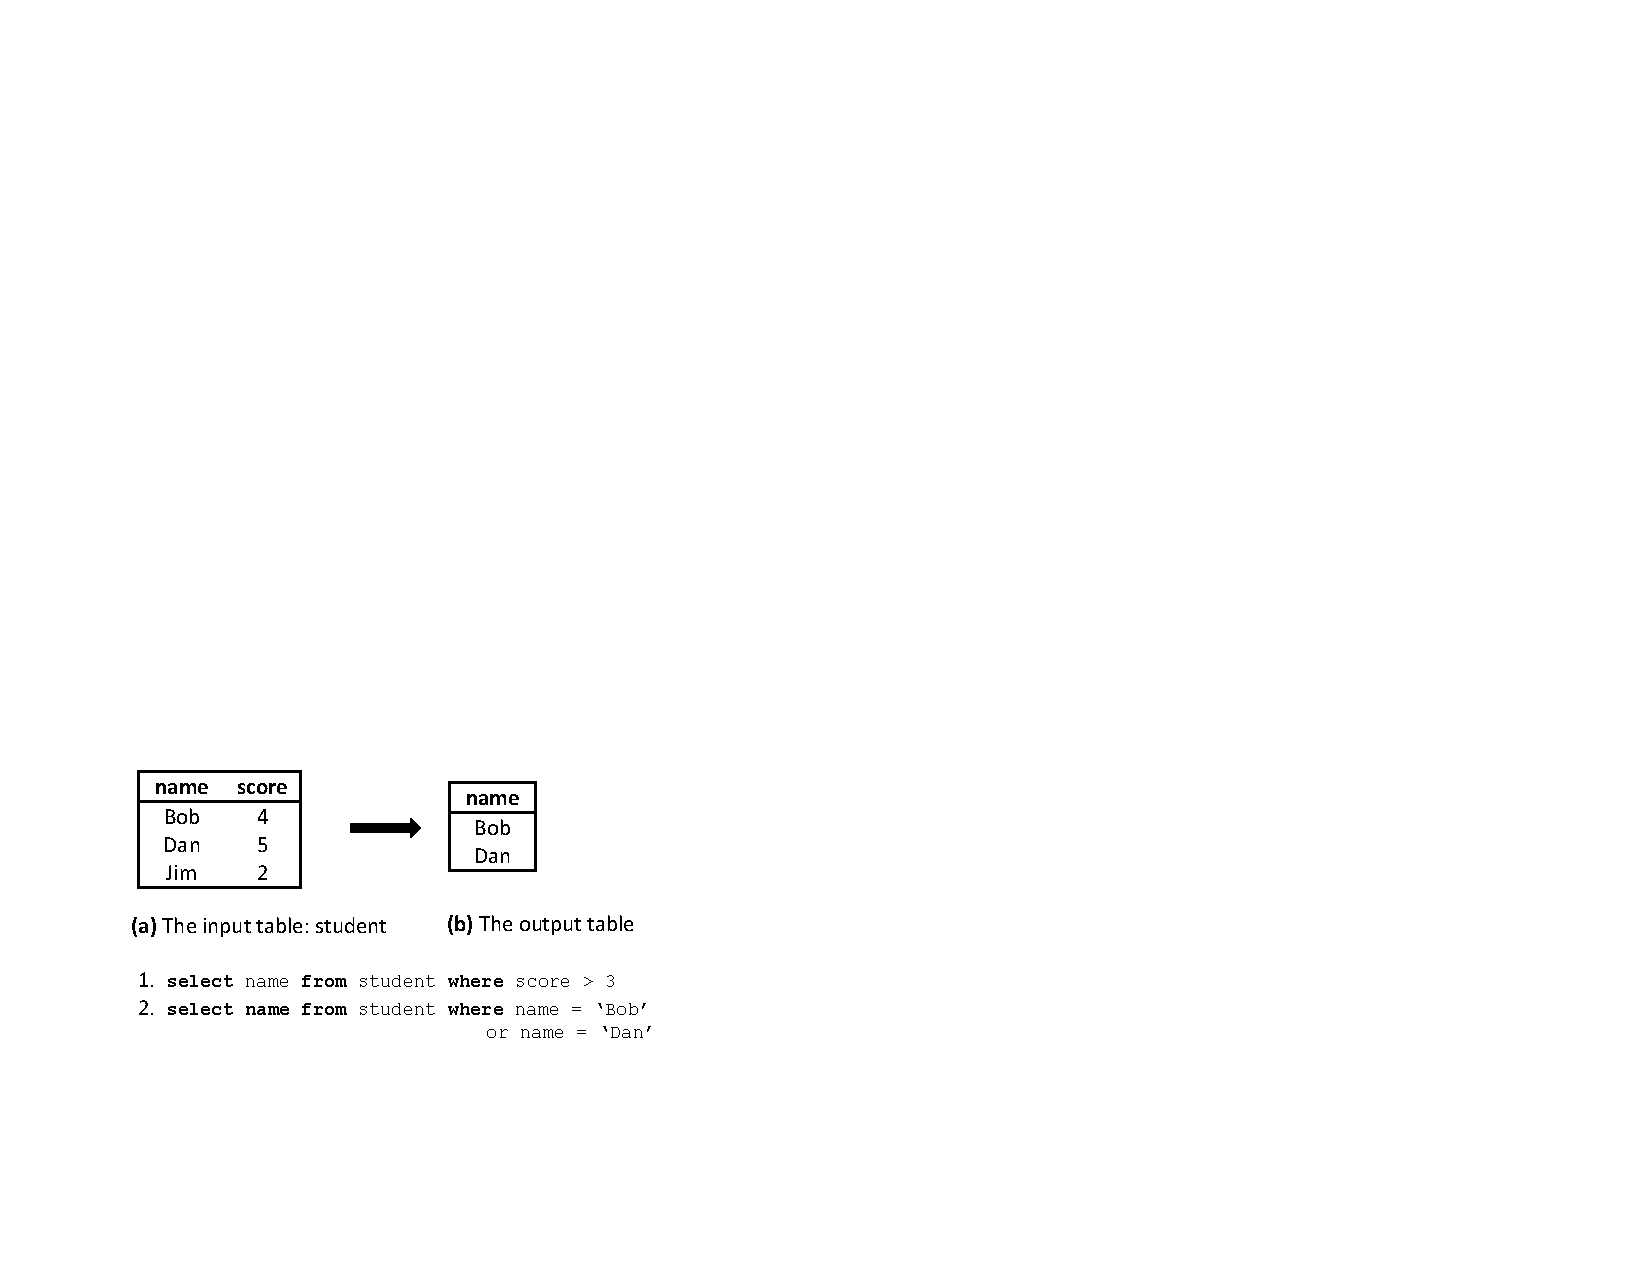
\includegraphics[scale=0.80]{rankexample}
 \vspace{-4mm}
\Caption{{\label{fig:rank} Illustration of \ourtool's
query ranking heuristic. \ourtool produces two
queries for the given examples. The first query
differs from the second query in using a simpler condition,
and thus is ranked higher.
}}
\end{figure}




%\subsection{User Interactive Model}
%\label{sec:uim}


